\documentclass[11pt]{article}

% Required packages:
\def\AssignmentMode{HW}     % HW | Lab | LabVIEW
\def\HWNum{2}
\def\AssignmentText{The Demonstration Check-Offs For Exercises 1 And 2 Are Due By \textcolor{red}{\HWCheckOffTime~\GetDate{4}{1}}. Check-Offs For Exercises 3 And 4 Are Due By \textcolor{red}{\HWCheckOffTime~\GetDate{5}{1}}. \\
Remainder Due On GradeScope, by \textcolor{red}{\HWSubmitTime~\GetDate{5}{2}}.}

% Course metadata
% ============================
% Required packages
% ============================

% \usepackage[letterpaper, total={6in, 9.5in}]{geometry}
\usepackage[
  letterpaper,
  left=0.5in,
  right=0.5in,
  top=0.5in,
  bottom=1.0in
]{geometry}


\usepackage[most]{tcolorbox}
\usepackage{booktabs}
\usepackage{fancyhdr}
\usepackage{graphicx}
\usepackage[
  colorlinks=true,
  linkcolor=blue,
  urlcolor=blue,
  citecolor=blue
]{hyperref}
\usepackage{lastpage}
\usepackage{listings}
\usepackage{minted}
\usepackage{setspace}
\usepackage{subcaption}
\usepackage{tabularx}
\usepackage{tikz}
\usepackage{xcolor}
\usepackage{xparse}
\usepackage[siunitx, american, RPvoltages]{circuitikz}
% Required packages:
\usepackage[table]{xcolor}
\usepackage{array}
\usepackage{array,colortbl,xcolor}
\usepackage{pdflscape}
\usepackage{pgfplots}
\usepackage{xurl}
\usetikzlibrary{arrows.meta, angles, quotes, shapes.symbols, arrows.meta}


\usepackage{pgfcalendar}

%%%%%%%%%%%%%%%%%%%% MODIFY DATES HERE %%%%%%%%%%%%%%%%

\def\Year{2026}
\def\StartDate{\Year-01-19}

\def\HWCheckOffTime{5PM}
\def\HWSubmitTime{9AM}
\def\LabVIEWSubmitTime{5PM}

%%%%%%%%%%%%%%%%%%%%%%%%%%%%%%%%%%%%%%%%%%%%%%%%%%%%%%%

\newcount\julianday
\newcount\myweekday % Define a counter for the weekday index

\newcommand{\GetDate}[2]{%
    \pgfcalendardatetojulian{\StartDate}{\julianday}%
    \advance\julianday by \numexpr #1*7 + #2\relax%
    % 1. Convert JDN to a date (sets \myyear, \mymonth, \myday)
    \pgfcalendarjuliantodate{\julianday}{\myyear}{\mymonth}{\myday}%
    % 2. Convert JDN to a weekday index 0..6 and store in \myweekday
    \pgfcalendarjuliantoweekday{\julianday}{\myweekday}%
    % 3. Print the name using the index, then the rest
    \pgfcalendarweekdayname{\myweekday}, \pgfcalendarmonthname{\mymonth} \myday%
}

\def\Final{\GetDate{16}{3}}
\usepackage{tikz}
\usepackage{xcolor}

\definecolor{iconGold}{RGB}{249,219,132}
\definecolor{iconGreen}{RGB}{71,160,93}

% Derived Border Colors (Darkened for contrast)
\definecolor{borderGold}{RGB}{180,150,80}
\definecolor{borderGreen}{RGB}{50,110,65}

\tikzset{
    ide_icon/.style={
        baseline=-0.3ex,
        line join=round,
        line cap=round,
        % Set a default border width that scales 
        line width=0.4pt 
    }
}

\newcommand{\pauseBtn}[1][0.4]{%
\begin{tikzpicture}[ide_icon, scale=#1]
    \filldraw[fill=iconGold, draw=borderGold] (0,0) rectangle (0.25, 0.8);
    \filldraw[fill=iconGold, draw=borderGold] (0.4,0) rectangle (0.65, 0.8);
\end{tikzpicture}}

\newcommand{\playBtn}[1][0.4]{%
\begin{tikzpicture}[ide_icon, scale=#1]
    \filldraw[fill=iconGold, draw=borderGold] (0,0) rectangle (0.15, 0.8);
    \filldraw[fill=iconGreen, draw=borderGreen] (0.25,0) -- (0.25,0.8) -- (0.75,0.4) -- cycle;
\end{tikzpicture}}

\newcommand{\debugBtn}[1][0.55]{%
\begin{tikzpicture}[ide_icon, scale=#1, rotate=45]
    % Legs: use border color for the stroke
    \draw[borderGreen, line width=0.6pt] (-0.3, 0.5) -- (0.3, 0.1);
    \draw[borderGreen, line width=0.6pt] (-0.3, 0.3) -- (0.3, 0.3);
    \draw[borderGreen, line width=0.6pt] (-0.3, 0.1) -- (0.3, 0.5);

    % Antenna
    \draw[borderGreen, line width=0.6pt] (0, 0.6) -- (-0.15, 0.75);
    \draw[borderGreen, line width=0.6pt] (0, 0.6) -- (0.15, 0.75);
    % Body
    \filldraw[fill=iconGreen, draw=borderGreen] (0,0.3) ellipse (0.18 and 0.25);
    % Head
    \filldraw[fill=iconGreen, draw=borderGreen] (0,0.6) circle (0.08);

\end{tikzpicture}}

\newcommand{\restartBtn}[1][0.8]{%
\begin{tikzpicture}[ide_icon, scale=#1]

    % Shaft with border
    \draw[borderGold, line width=1.8pt]
        (0,0.2) -- (0,0) -- (0.4,0) -- (0.4,0.2);

    \draw[iconGold, line width=1.0pt]
        (0,0.2) -- (0,0) -- (0.4,0) -- (0.4,0.2);

    % Arrowhead with proper outline
    \filldraw[
        fill=iconGold,
        draw=borderGold,
        line join=round
    ]
        (-0.1,0.2) -- (0.1,0.2) -- (0,0.33) -- cycle;

    % Green triangle cap
    \filldraw[fill=iconGreen, draw=borderGreen]
        (0.15,0.1) -- (0.15,0.5) -- (0.4,0.3) -- cycle;

\end{tikzpicture}%
}

% ============================
% Assignment mode resolution
% ============================

\def\CourseCode{SE 423}
\def\CourseName{Mechatronics}

\def\AssignmentType{}
\def\AssignmentFooter{}

\makeatletter
\@namedef{Assignment@HW@type}{Homework Assignment}
\@namedef{Assignment@HW@footer}{HW}

\@namedef{Assignment@Lab@type}{Laboratory Assignment}
\@namedef{Assignment@Lab@footer}{Lab}

\@namedef{Assignment@LabVIEW@type}{LabVIEW Assignment}
\@namedef{Assignment@LabVIEW@footer}{LabVIEW}

\@ifundefined{Assignment@\AssignmentMode @type}{
  \PackageError{AssignmentMode}{Invalid AssignmentMode}{%
    Valid options: HW, Lab, LabVIEW}
}{
  \edef\AssignmentType{\@nameuse{Assignment@\AssignmentMode @type}}
  \edef\AssignmentFooter{\@nameuse{Assignment@\AssignmentMode @footer}}
}
\makeatother

% ============================
% Header / footer
% ============================

\pagestyle{fancy}
\fancyhf{}
\fancyfoot[L]{// \CourseCode, \CourseName}
\fancyfoot[R]{// \AssignmentFooter~\HWNum, Page \thepage\ of \pageref{LastPage}}
\renewcommand{\headrulewidth}{0pt}

% ============================
% Title box
% ============================

\newcommand{\MakeAssignmentTitle}{
\begin{tcolorbox}[
    colback=gray!30!white,
    width=\textwidth,
    boxrule=0.8pt,
    arc=2mm,
    left=6mm,
    right=6mm,
    top=4mm,
    bottom=4mm,
    center
]
\centering
\setstretch{1.2}

\textbf{\Large \CourseCode\ \CourseName \\ \AssignmentType\ \#\HWNum}

\vspace{2mm}

\textbf{
\AssignmentText
}
\end{tcolorbox}
\vspace{0.5cm}
}

\setmintedinline{breaklines, breakafter=_}


\setminted{
  breaklines,
  breakanywhere=false,
  breakafter=\space,
  frame=lines,
  fontsize=\footnotesize,
}


\lstset{
    basicstyle=\ttfamily,   % Typewriter font for code
    breaklines=true,        % Allow breaking long lines
    columns=flexible        % Makes spacing better for inline
}

\newcounter{exercise}

\NewDocumentCommand{\Ex}{o}{
  \stepcounter{exercise}
  \section*{Exercise \theexercise
    \IfValueT{#1}{: #1} 
  }
  \addcontentsline{toc}{section}{Exercise \theexercise
    \IfValueT{#1}{: #1}}
}


\newcolumntype{C}[1]{>{\centering\arraybackslash}p{#1}}

\pgfplotsset{compat=1.18} 

%%%%%%%%%%%%%%%%%%%%%%%%%%%

\usepgfplotslibrary{groupplots}
\pgfplotsset{compat=1.17}


%%%%%%%%%%%%%%%%%%%%%%%%%%%
%
\begin{document}
\MakeAssignmentTitle

\Ex[Solder photo resistor]

Solder your breakout board to add the photo resistor circuit, connected to ADCINA4 (Pin 69) on the red board. Also, solder the 5-pin female header connector for your Joystick. See the Demo Board in the lab as a guide on what to solder to your board.
%
\begin{figure}[ht!]
\centering
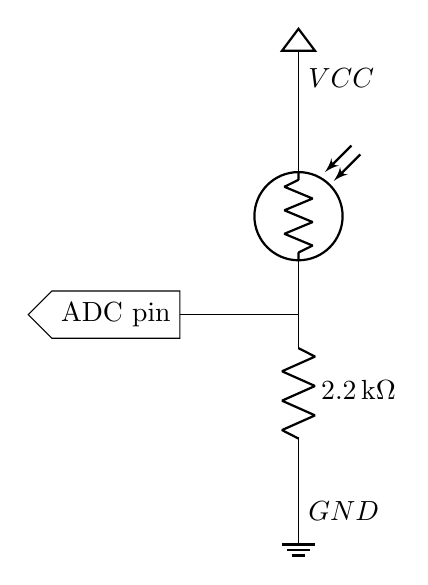
\begin{tikzpicture}

% Ground and VCC
\node[ground] (GND) at (0,0) {};
\node[sground, xscale=-1, yscale=-1] (VCC) at (0,5.5) {};

\node[anchor=west] at (GND.text) {$GND$};
\node[anchor=west] at (VCC.text) {$VCC$};

% Junction node (ADC sense point)
\coordinate (J) at (0,2.5);

% LDR (top)
\draw (J) to[american light dependent resistor, mirror] (0,5);

% Fixed resistor (bottom)
\draw (J) to[american resistor, l={$2.2\,\text{k}\Omega$}] (0,0.5);

% Connections to rails
\draw (0,5) -- (VCC);
\draw (0,0.5) -- (GND);

% ADC pin
\draw (J) -- (-1.5,2.5);
\node[
    draw,
    signal,
    signal to=left,
    signal from=none,
    fill=white,
    minimum height=0.6cm,
    anchor=east
] at (-1.5,2.5) {ADC pin};

\end{tikzpicture}
\caption{Photo resistor circuit}
\end{figure}
%
\Ex[Vary the intensity of an LED connected to a PWM output]

Create a new CCS project from the HWstarter project found in your repository and rename it \lstinline|HW2<yourinitials>|. Use this same project for all the exercises below. Each exercise builds on the next one.  
As discussed in the lecture, the EPWM peripheral has many more options than we will need for SE423 this semester. We only need to focus on the peripheral's basic features. I have created a condensed version of the EPWM chapter of the F28379D technical reference guide. The condensed version can be found here \url{http://coecsl.ece.illinois.edu/SE423/EPWM_Peripheral.pdf}. The complete technical reference guide can be found here \url{http://coecsl.ece.illinois.edu/SE423/tms320f28379D_TechRefi.pdf}.   
To set up the PWM peripheral and its output channels, you will need to program the PWM peripheral registers through the “bit-field” unions TI defined. Let us look at the definition of the bit-fields for the registers \mintinline{c}{TBCTL} and \mintinline{c}{AQCTLA}.  (\textbf{Note}: you can find these definitions in Code Composer Studio also by typing in the text \mintinline{c}{EPwm12Regs}, somewhere in your \lstinline|main()| function, and then right clicking and selecting “Open Declaration.”  Then do that one more time on the \lstinline|TBCTL_REG| union. YOU DO NOT cut and paste the code below into your code. I am just showing you how to view variable definitions using “Open Declaration”. Make sure to delete this single line of code where you typed \mintinline{c}{EPwm12Regs}, otherwise you will receive a compiler error later.)
%
\begin{minted}{c}
struct TBCTL_BITS {                     // bits description
    Uint16 CTRMODE:2;                   // 1:0 Counter Mode
    Uint16 PHSEN:1;                     // 2 Phase Load Enable
    Uint16 PRDLD:1;                     // 3 Active Period Load
    Uint16 SYNCOSEL:2;                  // 5:4 Sync Output Select
    Uint16 SWFSYNC:1;                   // 6 Software Force Sync Pulse
    Uint16 HSPCLKDIV:3;                 // 9:7 High Speed TBCLK Pre-scaler
    Uint16 CLKDIV:3;                    // 12:10 Time Base Clock Pre-scaler
    Uint16 PHSDIR:1;                    // 13 Phase Direction Bit
    Uint16 FREE_SOFT:2;                 // 15:14 Emulation Mode Bits
};
union TBCTL_REG {
    Uint16 all;
    struct TBCTL_BITS bit;
};

struct AQCTLA_BITS {                    // bits description
    Uint16 ZRO:2;                       // 1:0 Action Counter = Zero
    Uint16 PRD:2;                       // 3:2 Action Counter = Period
    Uint16 CAU:2;                       // 5:4 Action Counter = Compare A Up
    Uint16 CAD:2;                       // 7:6 Action Counter = Compare A Down
    Uint16 CBU:2;                       // 9:8 Action Counter = Compare B Up
    Uint16 CBD:2;                       // 11:10 Action Counter = Compare B Down
    Uint16 rsvd1:4;                     // 15:12 Reserved
};

union AQCTLA_REG {
    Uint16 all;
    struct AQCTLA_BITS bit;
};
\end{minted}
%
Looking at these bit-fields notice the \mintinline{c}{:1}, \mintinline{c}{:2} or \mintinline{c}{:3} after \mintinline{c}{PHSEN}, \mintinline{c}{CTRMODE}, \mintinline{c}{CLKDIV} respectively. This indicates how many bits this portion of the bit field uses. If you add up all the numbers after the colons, you see that it adds to 16, which is the size of both the \mintinline{c}{TBCTL} and \mintinline{c}{AQCTLA} registers. So each bit of the register can be assigned to this bit field. To make this clearer, look at the definition of \mintinline{c}{TBCTL} and \mintinline{c}{AQCTLA} from TI’s technical reference guide:
%
\begin{table}[H]
\caption{TBCTL Register: Figure 15-93}
\footnotesize
\centering
% \renewcommand{\arraystretch}{1.4}
% \setlength{\tabcolsep}{4pt}
\setlength{\tabcolsep}{0pt} % eliminate horizontal padding

% Color definitions (matched to figure)
\definecolor{bitbg}{RGB}{255,255,210}    % lighter yellow
%
\begin{tabular}{|*{8}{C{2cm}|}}

\hline

\rowcolor{bitbg}
15 & 14 & 13 & 12 & 11 & 10 & 9 & 8 \\
\hline

\multicolumn{2}{|c|}{FREE\_SOFT} &
\multicolumn{1}{c|}{PHSDIR} &
\multicolumn{3}{c|}{CLKDIV} &
\multicolumn{2}{c|}{HSPCLKDIV} \\
\hline

\multicolumn{2}{|c}{R/W-0h} &
\multicolumn{1}{c}{R/W-0h} &
\multicolumn{3}{c}{R/W-0h} &
\multicolumn{2}{c|}{R/W-1h} \\
\hline

\rowcolor{bitbg}
7 & 6 & 5 & 4 & 3 & 2 & 1 & 0 \\
\hline

\multicolumn{1}{|c|}{HSPCLKDIV} &
\multicolumn{1}{c|}{SWFSYNC} &
\multicolumn{2}{c|}{SYNCOSEL} &
\multicolumn{1}{c|}{PRDLD} &
\multicolumn{1}{c|}{PHSEN} &
\multicolumn{2}{c|}{CTRMODE} \\
\hline

\multicolumn{1}{|c|}{R/W-1h} &
\multicolumn{1}{c}{R-0/W1S-0h} &
\multicolumn{2}{c}{R/W-0h} &
\multicolumn{1}{c}{R/W-0h} &
\multicolumn{1}{c}{R/W-0h} &
\multicolumn{2}{c|}{R/W-3h} \\
\hline

\end{tabular}
\end{table}
%
and
%
\begin{table}[H]
\caption{AQCTLA Register: Figure 15-115}
\footnotesize
\centering
% \renewcommand{\arraystretch}{1.4}
% \setlength{\tabcolsep}{4pt}
\setlength{\tabcolsep}{0pt} % eliminate horizontal padding

% Color definitions (matched to figure)
\definecolor{bitbg}{RGB}{255,255,210}    % lighter yellow
%
\begin{tabular}{|*{8}{C{1.85cm}|}}

\hline

\rowcolor{bitbg}
15 & 14 & 13 & 12 & 11 & 10 & 9 & 8 \\
\hline


\multicolumn{4}{|c|}{\cellcolor{gray!30}RESERVED} &
\multicolumn{2}{c|}{CBD} &
\multicolumn{2}{c|}{CBU}  \\
\hline

\multicolumn{4}{|c}{R-0-0h} &
\multicolumn{2}{c}{R/W-0h} &
\multicolumn{2}{c|}{R/W-0h} \\
\hline

\rowcolor{bitbg}
7 & 6 & 5 & 4 & 3 & 2 & 1 & 0 \\
\hline

\multicolumn{2}{|c|}{CAD} &
\multicolumn{2}{c|}{CAU} &
\multicolumn{2}{c|}{PRD} &
\multicolumn{2}{c|}{ZRO} \\
\hline

\multicolumn{2}{|c}{R/W-0h} &
\multicolumn{2}{c}{R/W-0h} &
\multicolumn{2}{c}{R/W-0h} &
\multicolumn{2}{c|}{R/W-0h} \\
\hline

\end{tabular}
\end{table}
%
Notice that CLKDIV occupies 3 bits of the TBCTL register. CAU takes up 2 bits of the AQCTLA register. So, what bit-field unions allow us to do in our program is assign the value of the three CLKDIV bits without changing the other bits of the register. So you could code:
%
\begin{minted}{c}
EPwm12Regs.TBCTL.bit.CLKDIV = 3;
\end{minted}
%
Moreover, that would set bit 10 to 1, bit 11 to 1, and bit 12 to 0 in the TBCTL register, leaving all the other bits unchanged. Since CLKDIV uses 3 bits, the smallest value you can set it to is 0. What is the largest number you could set it to? \textit{(Technically, you could set it to any number in your code, but only the bottom 3 bits of the number are looked at in the assignment.)}  The answer is 7 or binary 111, all three bits set to 1.   

Given the introduction to register bit-field assignments, write some code in the \mintinline{c}{main()} function to set up EPWM12A to drive LED1. \textit{If I do not list an option that you see defined in a register, then that means you should not set that option, and it will be kept as the default. I may suggest an option that is already the default, but to make it clear to the reader of your code that this option is set, I would like you to assign it the default value, even though that line of code is not necessary.} Set the following options in the EPWM registers for EPWM12A:

With TBCTL set all these options using four lines of C code: (1) Count up Mode, (2) Free Soft emulation mode to Free Run so that the PWM continues when you set a break point in your code, (3) Do not load the time-base counter from the time-base phase register, (4) set clock divide to divide by 1. 

With TBCTR: Start the timer at zero.

With TBPRD: Set the period (carrier frequency) of the PWM signal to 5KHz, which is a period of 200 microseconds. Remember, the clock source the TBCTR register is counting has a frequency of 50 MHz, or a period of 1/50000000 seconds.  

With CMPA, initially start the duty cycle at 50%.  

With AQCTLA set, set the PWM12A output pin low when CMPA is reached. Set the pin high when the TBCTR register is zero.  

With TBPHS set to zero, i.e., \mintinline{c}{EPwm12Regs.TBPHS.bit.TBPHS = 0;} I do not know if this setting is necessary, but I have seen it in several TI examples, so I am just being safe here.  

You also need to set the PinMux so EPWM12A is used instead of GPIO22. Use the \href{http://coecsl.ece.illinois.edu/se423/hw/PinMuxTableF28379DLaunchPad.pdf}{PinMux table for the F28379D Launchpad} to help you here. Use the function \mintinline{c}{GPIO_SetupPinMux} to change the PinMux such that GPIO22 is instead set as EPWM12A output pin. For example, the below line of code sets GPIO158 as GPIO158: 
%
\begin{minted}{c}
GPIO_SetupPinMux(158, GPIO_MUX_CPU1, 0); //GPIO PinName, CPU, Mux Index
\end{minted}
%
Looking at the PinMux table, the line of code below sets GPIO40 to be instead the SDAB pin:
%
\begin{minted}{c}
GPIO_SetupPinMux(40, GPIO_MUX_CPU1, 6); //GPIO PinName, CPU, Mux Index   
\end{minted}
%
Finally, based on a number of TI examples, it is a good idea to disable the pull-up resistor when an I/O pin is set as a PWM output to reduce power consumption. Add these lines of code after your above initializations.  
%
\begin{minted}{c}
EALLOW;  // Below are protected registers
GpioCtrlRegs.GPAPUD.bit.GPIO22 = 1; // For EPWM12A
EDIS;
\end{minted}
%
Compile your code and fix any compiler errors. So that you can see LED1 dimming and brightening, go to CPU Timer 0’s interrupt function and comment out the call to the \mintinline{c}{displayLEDletter()} function. When ready, download this code to your Launchpad. When you run your code, the EPWM12A signal driving LED1 is 50\% duty cycle, so the LED should be 50\% on. You will change the duty cycle of EPWM12A by manually updating its CMPA register in Code Composer Studio. In CCS, select the menu View -> Registers, and the Registers tab should appear. There are a bunch of registers, so you will have to scroll down until you see the “EPwm12Regs” register. Click the “$>$” to expand the register. Scroll down until you find the TBPRD and CMPA registers. Note the value in TBPRD. Expand the CMPA register and confirm that it is a 32-bit register with two 16-bit parts, CMPA and CMPAHR. Leave CMPAHR at 0 and change CMPA. First, try setting CMPA to 3/4 the value of TBPRD. What happens to the intensity of LED1? Change CMPA to the same value as TBPRD to see the maximum brightness (100\% duty cycle). Play with other values for CMPA to see the brightness change.  

\textbf{Note}: Code Composer Studio may not display your EPWM12 registers correctly due to very little code running on your F28379D processor, and also due to the large number of registers to display in the register view. Once you click the Registers tab, you will see two icons with yellow arrows pointing towards each other. These are Refresh and Continuous Refresh. When you enter a value for CMPA, try clicking Refresh and Continuous Refresh to see if CCS refreshes the value in CMPA. If the Refresh icons do not work, you can also pause your code with the pause icon, and your values should update. Then click the resume icon to continue running your code.  

Now that you see CMPA changes the brightness of LED1, initialize CPU Timer 2 so that its interrupt function is called every 1ms. Then write code in CPU Timer2’s interrupt function to increase, by one, the value of EPWM12’s CMPA register every one millisecond. Then, when CMPA’s value reaches the value in TBPRD, change the state of your code to decrease CMPA by 1 each millisecond; then, when CMPA reaches 0, start increasing CMPA by 1 again each millisecond. This way, your code will change the duty cycle of the PWM driving LED1, making it brighter, then dimmer, and repeating this process. The easiest way to code this is to create a global variable of type \mintinline{c}{int16_t} named updown. When updown is equal to 1, count up; when updown is 0, count down. When counting, check for CMPA to reach the value of TBPRD and switch to down counting. While down-counting, check if CMPA equals zero to switch back to up-counting.
%
\begin{figure}[H]
    \centering
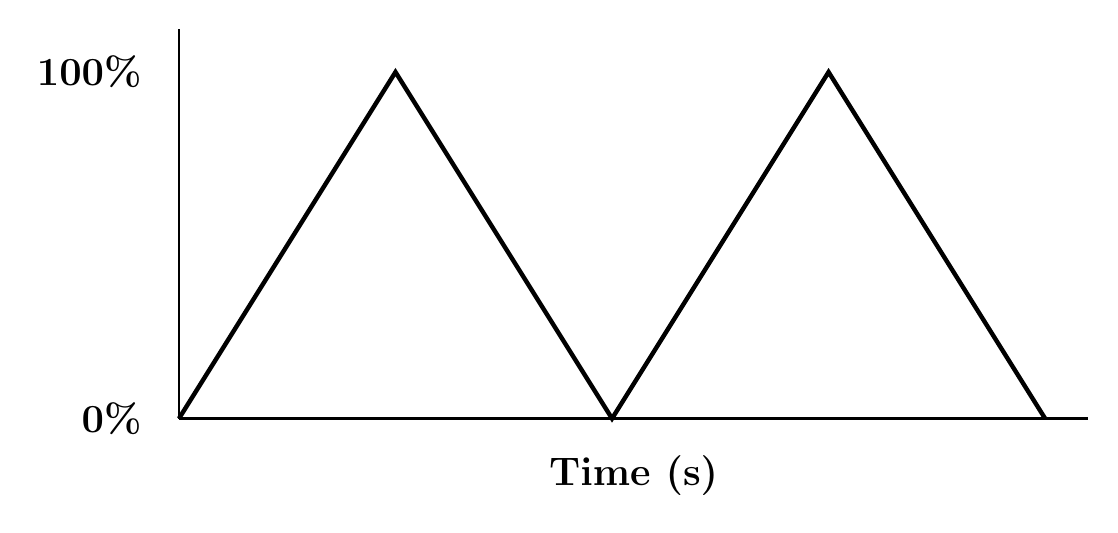
\begin{tikzpicture}[scale=1.1]

    % Axes
    \draw[thick] (0,0) -- (10.5,0); % x-axis
    \draw[thick] (0,0) -- (0,4.5);  % y-axis

    % Axis labels
    \node[below=10pt] at (5.25,0) {\Large\textbf{Time (s)}};
    \node[left=10pt] at (0,0) {\Large\textbf{0\%}};
    \node[left=10pt] at (0,4) {\Large\textbf{100\%}};

    % Triangular waveform
    \draw[ultra thick]
        (0,0) --
        (2.5,4) --
        (5,0) --
        (7.5,4) --
        (10,0);
\end{tikzpicture}
    \caption{Ramped LED1 Brightness Pattern}
\end{figure}
%
\Ex[Using ADCA to read the voltage drop across a photo resistor]

These documents will help you understand how to use the ADC peripheral. Find the whole chapter 11 discussing the F28379D’s ADC peripheral in the \href{http://coecsl.ece.illinois.edu/se423/tms320f28379D_TechRefi.pdf}{TMS320F28379D Technical Reference Guide} just in case you need some extra detail. Also, read through sections 3.4 through 3.4.5, which discuss Hardware Interrupt events on the F28379D. \href{http://coecsl.ece.illinois.edu/se423/PeripheralInterruptChannelMapTable.pdf}{Table 3-2} is important when setting up Hardware Interrupts (HWI), so I have created a separate file with that table only. I have created a condensed version of the ADC peripheral that should cover most of the topics we need for this homework. 
\href{http://coecsl.ece.illinois.edu/se423/ADC_Peripheral.pdf}{ADC Condensed Technical Reference Guide}. These included sections and register descriptions, which should give you an introduction to the ADC peripheral. The EPWM4 peripheral will be used to signal the ADC when to convert, rather than driving a duty-cycle-varying square wave, so I am including another link to the EPWM reference here. \href{http://coecsl.ece.illinois.edu/se423/EPWM_Peripheral.pdf}{EPWM Condensed Technical Reference Guide}.

Each of the TMS320F28379D processor’s ADC peripherals can generate an interrupt when its sequence of samples has been converted and stored in the results registers of the ADC peripheral. When the ADC conversion is complete, the F28379D will automatically stop the code it is currently processing and jump to the interrupt service routine (ISR) specified for the ADC. Upon completion of the ISR code, the program counter (PC) will automatically jump back to the interrupted code and resume processing.  

There are four ADC peripherals in the F28379D: ADCA, ADCB, ADCC, and ADCD. For this first exercise with the ADC, we will use ADCA and its channel ADCINA4, which you have soldered to the photo resistor's output.  

The input pins, or channels, ADCINA0, ADCINA1, ADCINA2, ADCINA3, ADCINA4, and ADCINA5 are multiplexed into the ADCA peripheral on the F28379D processor. The ADCA peripheral can only sample one of these voltage input pins at a time. So the multiplexer allows the ADCA sequencer to sample one channel, and then, when finished, the sequencer can change the multiplexer so that the next channel can be converted. The sequencer can schedule up to 16 conversions for each trigger. At first, you will only set up one conversion, ADCINA4. However, in the next exercise, you will add channels to sample the voltage from your attached Joystick.  
We will initialize ADCA to perform 12-bit ADC conversions. The input voltage range for this ADC is 0 to 3.0 volts. So, a 12-bit result of 0 (decimal) indicates that 0.0 volts is on the ADC input pin. The maximum value of a 12-bit ADC result, 4095, indicates that almost 3.0 volts is on the ADC input pin. Hence, there is a linear interpolation between 0 and 4095, covering all voltages from 0.0 to almost 3.0 volts with steps of 3.0V/4096 = 0.73 mV. (The reason for 4096 here is due to how a SAR ADC is constructed.)
We will command ADCA to sample channel ADCINA4, which will be a one-channel sequence. (As I stated above, in the next exercise, you will also sample the two voltages of the Joystick and use a three-channel sequence.)  We will set up Start of Conversion 0 (SOC0) to convert ADCINA4. When SOC0 finishes converting the input voltage to its corresponding 12-bit value, the ADCA1 hardware interrupt will be flagged for execution. You will write the hardware interrupt function that is called when ADCA1 is flagged. The conversion results will be stored in the AdcaResultRegs registers.ADCRESULT0.     
There are quite a few things to set up, so I am giving you most of the code. You will need to refer to the register descriptions to fill in the blanks. I also include some commented-out code that will help you with the next exercise.  

We want to command the ADCA peripheral to sample ADCINA4. There are a few ways to accomplish this, but for this homework, we are going to use EPWM4 as a timer (no duty-cycle output) to trigger the ADCA conversion sequence. In \mintinline{c}{main()} after the \mintinline{c}{init_serial} functions, add the following code and fill in the ??? blanks by studying the EPWM reference. Do not forget to copy EALLOW and EDIS.   
%
\begin{minted}{c}
EALLOW;
EPwm4Regs.ETSEL.bit.SOCAEN = 0; // Disable SOC on A group
EPwm4Regs.TBCTL.bit.CTRMODE = 3; // freeze counter
EPwm4Regs.ETSEL.bit.SOCASEL = ???; // Select event when counter equal to PRD
EPwm4Regs.ETPS.bit.SOCAPRD = ???; // Generate pulse on 1st event (“pulse” is the same as “trigger”)

EPwm4Regs.TBCTR = 0x0; // Clear counter
EPwm4Regs.TBPHS.bit.TBPHS = 0x0000; // Phase is 0
EPwm4Regs.TBCTL.bit.PHSEN = 0; // Disable phase loading
EPwm4Regs.TBCTL.bit.CLKDIV = 0; // divide by 1 50Mhz Clock
EPwm4Regs.TBPRD = ???;  // Set Period to 1ms sample. The input clock is 50MHz.
// Notice here that we are not setting CMPA or CMPB because we are not using the PWM signal
EPwm4Regs.ETSEL.bit.SOCAEN = 1; //enable SOCA
EPwm4Regs.TBCTL.bit.CTRMODE = ???; //unfreeze, and enter up count mode
EDIS;
\end{minted}
%
Next, we would like to set up ADCA so that it uses 1 of its 16 SOCs (Start of Conversions). The ADC sequencer uses these SOCs to sample the ADC channels in any desired order and, if necessary, assign priority to certain SOCs. It may not be very clear for the first-time user of this peripheral, but if we stick to the basics, it is pretty straightforward. We will trigger SOC0 using the EPWM PRD time event. When triggered, SOC0 will sample/convert its assigned channel. Assign channel ADCINA4 to SOC0. The initializations below set up ADCA to flag an interrupt when SOC0 finishes converting. 

Some of the given code I found in an ADC example. It retrieves the default calibration values for the ADCA from the F28379D’s read-only memory (ROM). Add the following to \mintinline{c}{main()} after the \mintinline{c}{init_serial} functions, filling in the appropriate blanks (???). Note that the lines of C code that are commented out will be used in the next exercise when you also convert the Joystick channels.  
%
\begin{minted}{c}
EALLOW;
//write configurations for ADCA
AdcaRegs.ADCCTL2.bit.PRESCALE = 6; //set ADCCLK divider to /4
AdcSetMode(ADC_ADCA, ADC_RESOLUTION_12BIT, ADC_SIGNALMODE_SINGLE);  //read calibration settings
//Set pulse positions to late
AdcaRegs.ADCCTL1.bit.INTPULSEPOS = 1;
//power up the ADCs
AdcaRegs.ADCCTL1.bit.ADCPWDNZ = 1;
//delay for 1ms to allow ADC time to power up
DELAY_US(1000);

//Select the channels to convert and the end of conversion flag
//ADCA
AdcaRegs.ADCSOC0CTL.bit.CHSEL = ???; //SOC0 will convert Channel you choose Does not have to be A0
AdcaRegs.ADCSOC0CTL.bit.ACQPS = 99; //sample window is acqps + 1 SYSCLK cycles = 500ns
AdcaRegs.ADCSOC0CTL.bit.TRIGSEL = ???; // EPWM4 ADCSOCA 

//AdcaRegs.ADCSOC1CTL.bit.CHSEL = ???; //SOC1 will conv Channel you choose Does not have to be A1
//AdcaRegs.ADCSOC1CTL.bit.ACQPS = 99; //sample window is acqps + 1 SYSCLK cycles = 500ns
//AdcaRegs.ADCSOC1CTL.bit.TRIGSEL = ???; // EPWM4 ADCSOCA 

//AdcaRegs.ADCSOC2CTL.bit.CHSEL = ???; //SOC2 will conv Channel you choose Does not have to be A2
//AdcaRegs.ADCSOC2CTL.bit.ACQPS = 99; //sample window is acqps + 1 SYSCLK cycles = 500ns
//AdcaRegs.ADCSOC2CTL.bit.TRIGSEL = ???; // EPWM4 ADCSOCA 

AdcaRegs.ADCINTSEL1N2.bit.INT1SEL=???; //set to last or only SOC that is converted, and it will set INT1 flag ADCA1
AdcaRegs.ADCINTSEL1N2.bit.INT1E = 1; //enable INT1 flag
AdcaRegs.ADCINTFLGCLR.bit.ADCINT1 = 1; //make sure INT1 flag is cleared	
EDIS;
\end{minted}
%
\textbf{Note}: \textit{The naming can get confusing here. There are ADCA inputs channels labeled ADCINA0, ADCINA1, ADCINA2, ADCINA3, ADCINA4, ADCINA5 and there are also four ADCA interrupts labeled ADCA1, ADCA2, ADCA3 and ADCA4. In the above code, the ADCA1 interrupt is configured to trigger when channel ADCINA4 finishes conversion.}  You will be adding most of the remainder of your code for this exercise inside this ADCA1 hardware interrupt function.

Now add this ADCA1 hardware interrupt function. To get you started with this interrupt function, cut and paste this shell function somewhere in your code outside of your \mintinline{c}{main()} function.
%
\begin{minted}{c}
//adca1 pie interrupt
__interrupt void ADCA_ISR (void)
{
    Adca4result = AdcaResultRegs.ADCRESULT0;
    
    // Here covert ADCINA4 to volts

    // Print ADCINA4’s voltage value to TeraTerm every 100ms by setting UARTPrint to one every 100th 
    //time in this function.

    AdcaRegs.ADCINTFLGCLR.bit.ADCINT1 = 1;  //clear interrupt flag
    PieCtrlRegs.PIEACK.all = PIEACK_GROUP1;
}
\end{minted}
%
Furthermore, perform the following steps (\textit{some of these steps have already been done for you by the shell code}):
%
\begin{enumerate}
    \item Create your interrupt function as a global function with “\mintinline{c}{void}” parameters and of type “\mintinline{c}{__interrupt void}”, for example \mintinline{c}{__interrupt void ADCA_ISR(void) }  
    \item Put a predefinition of your ISR function at the top of your C file in the same area as the predefinitions of the CPU Timer ISRs.  
    \item Now inside \mintinline{c}{main()} find the \mintinline{c}{PieVectTable} assignments. This is how you tell the F28379D processor to call your defined functions when certain interrupt events occur. Looking at Table 3-2 in the \href{http://coecsl.ece.illinois.edu/se423/PeripheralInterruptChannelMapTable.pdf}{F28379d Technical Reference}, find ADCA1. You should see that it is PIE interrupt 1.1. Since TI labels this interrupt \mintinline{c}{ADCA1}, there is a \mintinline{c}{PieVectTable} field named \mintinline{c}{ADCA1_INT}. So inside the \mintinline{c}{EALLOW} and \mintinline{c}{EDIS} statement assign \mintinline{c}{PieVectTable.ADCA1_INT} to the memory address location of your ISR function. For example \mintinline{c}{&ADCA_ISR}.
    \item Next step is to enable the PIE interrupt 1.1 that the F28379D associated with ADCA1. Further down in the \mintinline{c}{main()} code, find the section of code of “\mintinline{c}{IER |=}” statements. This code enables the base interrupt for multiple PIE interrupts. Since ADCA1 is part of interrupt INT1, INT1 must be enabled. Timer 0’s interrupt is also a part of interrupt 1. So, the code we need is already there “\mintinline{c}{IER |= M_INT1;}”. You do, though, need to enable the 1st interrupt source of interrupt 1. Below the “\mintinline{c}{IER |=}” statements you should see the enabling of \mintinline{c}{TINT0} which is \mintinline{c}{PIEIER1.bit.INTx7}. Do the same line of code, but enable PIE interrupt 1.1.
    \item Now with everything set up to generate the ADCA1 interrupt, put code in your ADCA1 interrupt function to read the value of the ADCINA4. ADCINA4 is set up to convert the input voltage on its corresponding pin to a 12-bit integer. The ADC input range is 0.0V to almost 3.0V. The 12-bit conversion value, which ranges from 0 to 4095, linearly represents the input voltage from 0.0V to almost 3.0V. The 12-bit conversion value is stored in the results register, see the given code below. Create a global \mintinline{c}{int16_t} result variable to store ADCINA4’s “raw” reading. Create one global float variable to store the scaled (0V-3V) voltage value of ADCINA4. Write code to convert the ADCINA4 12-bit integer result value to voltage using the scale factor 3.0/4096.0 and store it in this global float variable. (The reason for 4096 here is due to how a SAR ADC is constructed.)     
    \item Set \mintinline{c}{UARTPrint = 1} every 100ms and change the code in the \mintinline{c}{main()} while loop so that your ADC voltage value is printed to TeraTerm. Make sure to create your own \mintinline{c}{int32_t} count variable for this ADA1 interrupt function. It is not a good idea to use a count variable from a different timer function.  
    \item As a final step, clear the interrupt source flag and the PIE peripheral so that the processor will wait for the next interrupt flag before the ADC ISR is called again. The code below has many of these steps. 
\end{enumerate}
%
Place your hand over the photo resistor and use a flashlight to observe the voltage output of your photo resistor circuit change. In addition, write code set EPWM12A’s CMPA register to a scaled value of the photo resistor’s reading. When the photoresistor is not receiving much light, LED1 should be dim. As the photoresistor sees more light, LED1 should get brighter due to the change in duty cycle.

Demonstrate these items working for your check off.  

\Ex[Also sample the Joystick voltages]

In this exercise, I would like you to add to the ADCA sequence of conversions by sampling the X- and Y-axis voltages of the Joystick. The Joystick X axis is connected to ADCINA2, and the Y axis is connected to ADCINA3. You will only have to make a few changes to Exercise 3’s code to make these additional samples occur. Leave SOC0 setup to sample ADCINA4 and triggered by EPWM4. Set up SOC1 to sample ADCINA2 and triggered by EPWM4, and SOC2 to sample ADCINA3 and triggered by EPWM4. Also, make sure to set the interrupt select so that SOC2 is the last sampled conversion and triggers the ADCA1 interrupt function. Then, inside the ADCA1 interrupt function, sample all three results, convert each to a voltage value between 0V and 3V, and print these three values to Tera Term every 100ms.  

Using the readings of the Joystick X and Y, write code to update LEDs to point in the direction you have moved the Joystick. If Joystick X is in the center position, turn on only LED8. If Joystick X is moved past a threshold and pointing towards the buzzer, then turn on only LED6. If Joystick X is moved past another threshold and pointing away from the buzzer, then turn on only LED10. Similarly, if Joystick Y is in the center position, turn on only LED8 if Joystick Y is moved past a threshold, and, pointing down, turn on only LED13. Suppose Joystick Y is moved past a threshold and pointing up, then only LED3 turns on. Demonstrate these items working for your check off.

\Ex[SPI timing diagram]

Answer the following questions about the SPI timing diagram on the next page. Remember that SPI both sends and receives data simultaneously.
%
\begin{enumerate}
    \item How many bytes are sent? How many bytes are received? What are the values of the bytes sent from the master to the slave? What are the values of the bytes received into the master from the slave?
    \item Approximate the bit rate (baud rate) by looking at the X-axis time divisions.  
    \item Look at Figure 18-7 and Figure 18-11 in the \href{http://coecsl.ece.illinois.edu/se423/SPICondensed_TechRef.pdf}{SPI Condensed Reference}. What SPI mode is being used in the below timing diagram: \mintinline{c}{CLOCK_POLARITY = ?}, \mintinline{c}{CLOCK_PHASE = ?}. So this means that the master reads in each bit on the rising edge of the clock (SCK) or the falling edge of SCK?  
\end{enumerate}
%
\begin{landscape}

% \begin{figure}
%     \centering
% \begin{tikzpicture}[scale=1.4]
% \definecolor{mosired}{RGB}{219,85,72}
% \definecolor{misoblue}{RGB}{84,153,207}
% \definecolor{sckorange}{RGB}{242,196,95}
% \definecolor{sspurple}{RGB}{167,123,181}

% \pgfmathsetmacro{\bit}{1/30}

% \begin{groupplot}[
%     group style={
%         group size=1 by 4, 
%         vertical sep=0.4cm,
%         x descriptions at=edge bottom
%     },
%     width=16cm,
%     height=3.5cm,
%     xmin=0, xmax=3.5,
%     ymin=-0.2, ymax=1.2,
%     % Use ytick for internal labels
%     ytick={0,1},
%     yticklabels={GND, 3.3V},
%     yticklabel style={font=\tiny, anchor=east},
%     % Grid settings
%     grid=both,
%     grid style={dotted, gray!60},
%     minor x tick num=14, % 5 subdivisions per 0.5 unit
%     xtick={0,0.5,1,1.5,2,2.5,3,3.5},
%     xlabel style={font=\small},
%     ylabel style={rotate=-90, font=\bfseries, anchor=south, xshift=-4ex}
% ]

% % --- MOSI Plot ---
% \nextgroupplot[title={\textbf{SPI Timing Diagram Analysis}}, ylabel={MOSI}]
% \addplot[const plot, no markers, mosired, very thick] coordinates {
%   (0,1)
%   (7*\bit,0)(9*\bit, 1)
%   (13*\bit,0)(15*\bit, 1)
%   (17*\bit,0)(19*\bit, 1)
%   (23*\bit,0)(31*\bit, 1)
%   (35*\bit,0)(37*\bit, 1)
%   (51*\bit,0)(59*\bit, 1)
%   (63*\bit,0)(71*\bit, 1)
%   (75*\bit,0)(79*\bit, 1)
%   (83*\bit,0)(85*\bit, 1)
%   (89*\bit,0)(93*\bit, 1)
%   (105*\bit, 1)
% };

% % --- MISO Plot ---
% \nextgroupplot[ylabel={MISO}]
% \addplot[const plot, no markers, misoblue, very thick] coordinates {
%   (0,1)
%   (2*\bit,0)(7*\bit, 1)
%   (11*\bit,0)(19*\bit, 1)
%   (22*\bit,0)(29*\bit, 1)
%   (31*\bit,0)(33*\bit, 1)
%   (48*\bit,0)(50*\bit, 1)
%   (52*\bit,0)(56*\bit, 1)
%   (63*\bit,0)(77*\bit, 1)
%   (85*\bit,0)(90*\bit, 1)
%   (94*\bit,0)(98*\bit, 1)
%   (105*\bit, 1)
% };

% % --- SCK Plot (Clock Signal) ---
% \nextgroupplot[ylabel={SCK}]
% \addplot[const plot, no markers, sckorange, very thick] coordinates {
%     (0,1) 
%     (3*\bit,0) (4*\bit,1)
%     (5*\bit,0) (6*\bit,1)
%     (7*\bit,0) (8*\bit,1)
%     (9*\bit,0) (10*\bit,1)
%     (11*\bit,0) (12*\bit,1)
%     (13*\bit,0) (14*\bit,1)
%     (15*\bit,0) (16*\bit,1)
%     (17*\bit,0) (18*\bit,1)

%     (18*\bit,1) (23*\bit,1)
%     (23*\bit,0) (24*\bit,1)
%     (25*\bit,0) (26*\bit,1)
%     (27*\bit,0) (28*\bit,1)
%     (29*\bit,0) (30*\bit,1)
%     (31*\bit,0) (32*\bit,1)
%     (33*\bit,0) (34*\bit,1)
%     (35*\bit,0) (36*\bit,1)
%     (37*\bit,0) (38*\bit,1)

%     (38*\bit,1) (43*\bit,1)
%     (43*\bit,0) (44*\bit,1)
%     (45*\bit,0) (46*\bit,1)
%     (47*\bit,0) (48*\bit,1)
%     (49*\bit,0) (50*\bit,1)
%     (51*\bit,0) (52*\bit,1)
%     (53*\bit,0) (54*\bit,1)
%     (55*\bit,0) (56*\bit,1)
%     (57*\bit,0) (58*\bit,1)

%     (58*\bit,1) (63*\bit,1)
%     (63*\bit,0) (64*\bit,1)
%     (65*\bit,0) (66*\bit,1)
%     (67*\bit,0) (68*\bit,1)
%     (69*\bit,0) (70*\bit,1)
%     (71*\bit,0) (72*\bit,1)
%     (73*\bit,0) (74*\bit,1)
%     (75*\bit,0) (76*\bit,1)
%     (77*\bit,0) (78*\bit,1)

%     (78*\bit,1) (83*\bit,1)
%     (83*\bit,0) (84*\bit,1)
%     (85*\bit,0) (86*\bit,1)
%     (87*\bit,0) (88*\bit,1)
%     (89*\bit,0) (90*\bit,1)
%     (91*\bit,0) (92*\bit,1)
%     (93*\bit,0) (94*\bit,1)
%     (95*\bit,0) (96*\bit,1)
%     (97*\bit,0) (98*\bit,1)

%     (98*\bit,1) (103*\bit,1)
%     (103*\bit,0) (104*\bit,1)
%     (105*\bit,0) (106*\bit,1)
%     (107*\bit,0) (108*\bit,1)
% };

% % --- SS Plot (Slave Select - Active Low) ---
% \nextgroupplot[ylabel={SS}, xlabel={$t$ (seconds $\times 10^{-5}$)}]
% \addplot[const plot, no markers, sspurple, very thick] coordinates {
%     (0,1) 
%     (2*\bit,0) (19*\bit,1)
%     (22*\bit,0) (39*\bit,1)
%     (42*\bit,0) (59*\bit,1)
%     (62*\bit,0) (79*\bit,1)
%     (82*\bit,0) (99*\bit,1)
%     (102*\bit,0) (119*\bit,1)
% };

% \end{groupplot}
% \end{tikzpicture}
%     \caption{SPI Timing Diagram Analysis}
%     \label{fig:spi}
% \end{figure}

\begin{figure}
    \centering
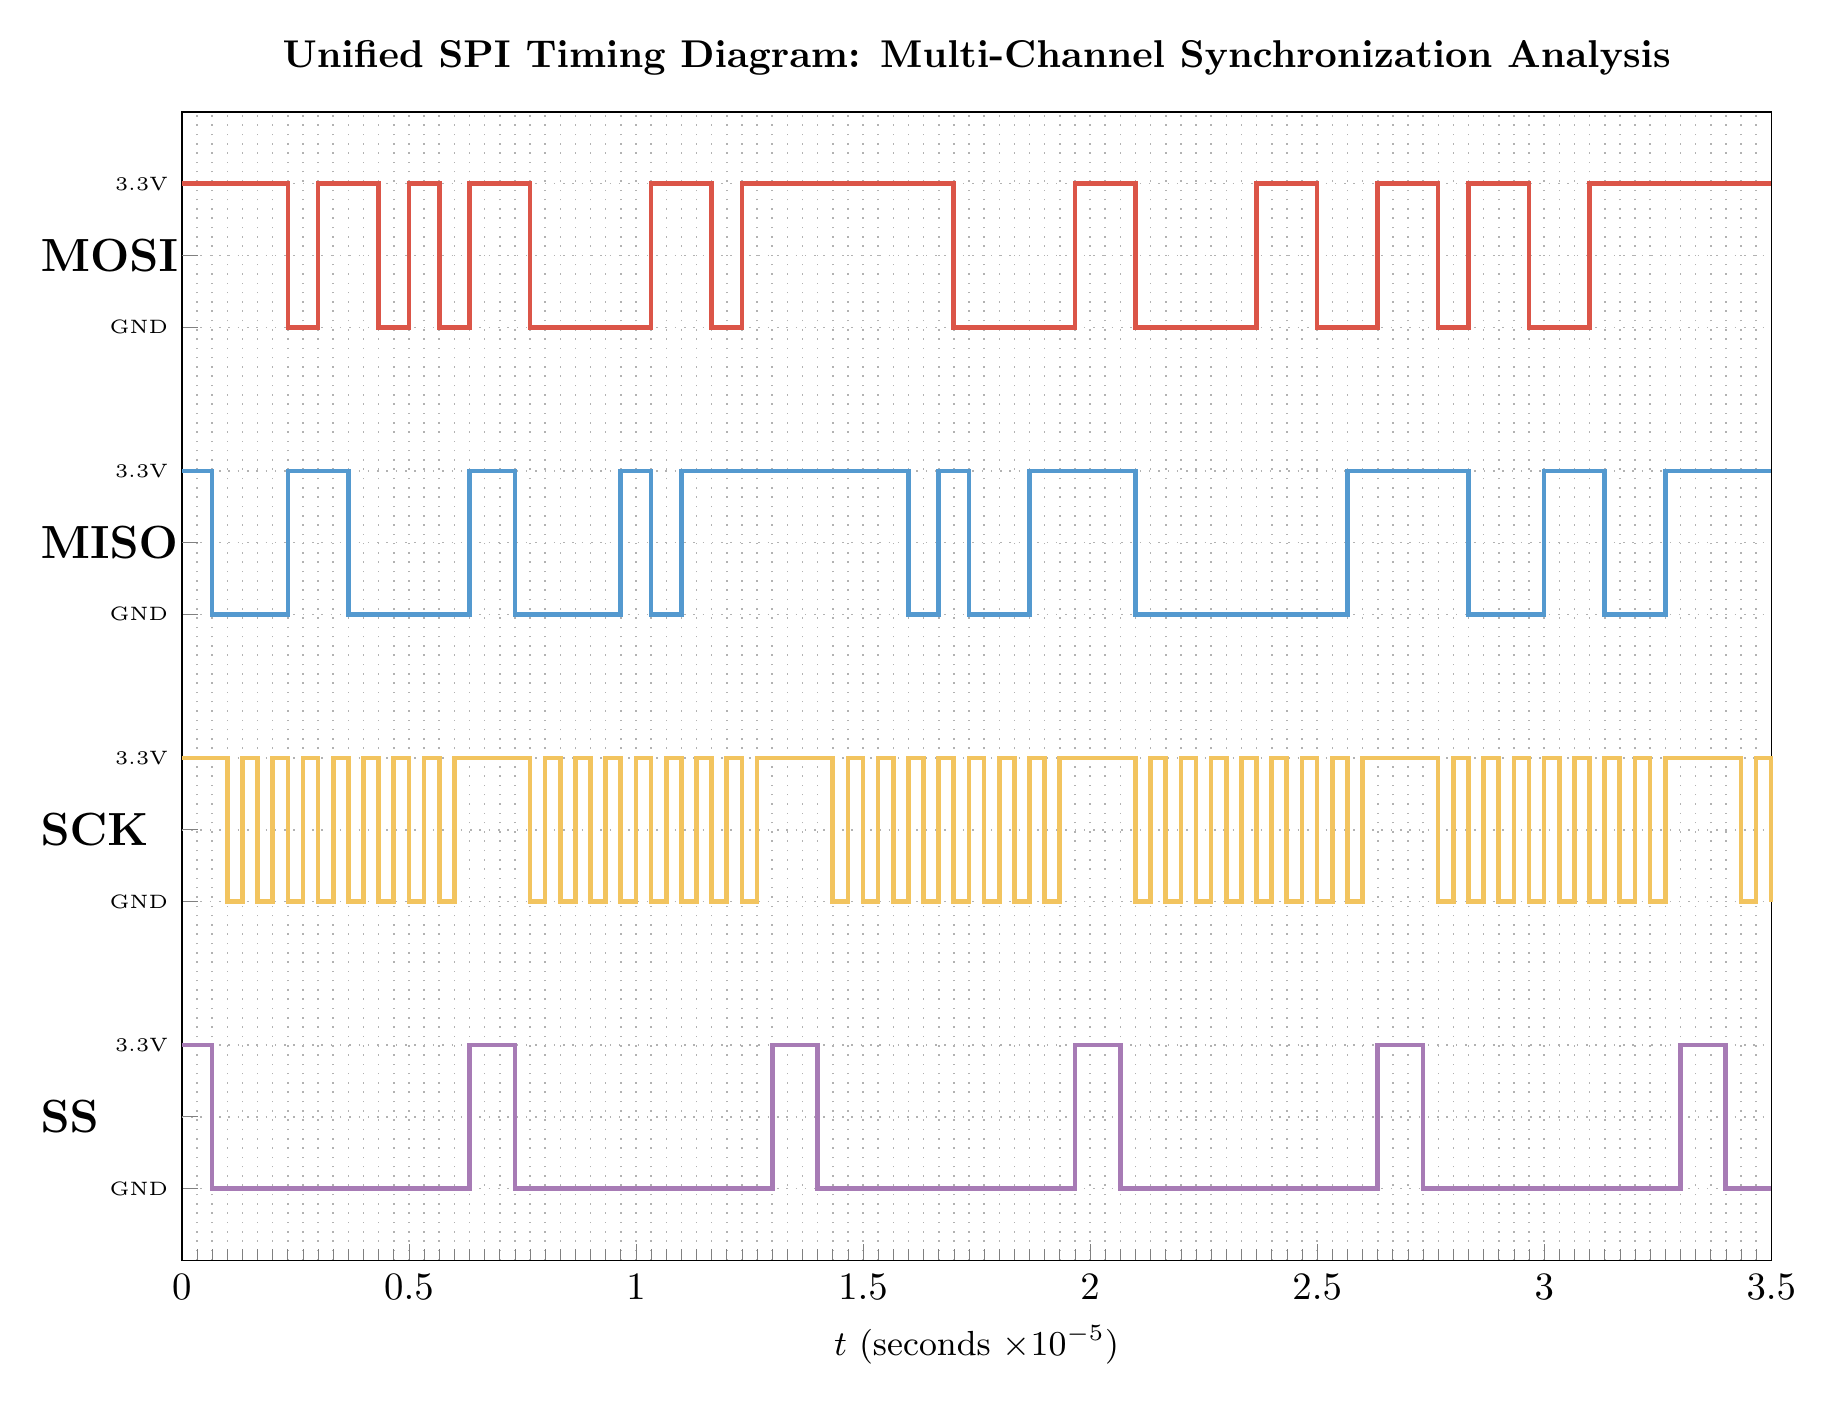
\begin{tikzpicture}[scale=1.4]
% Custom color palette for high-contrast signal differentiation
\definecolor{mosired}{RGB}{219,85,72}
\definecolor{misoblue}{RGB}{84,153,207}
\definecolor{sckorange}{RGB}{242,196,95}
\definecolor{sspurple}{RGB}{167,123,181}

\pgfmathsetmacro{\bit}{1/30}

\begin{axis}[
    width=16cm,
    height=12cm,
    xmin=0, xmax=3.5,
    ymin=-0.5, ymax=7.5,
    % Primary Y-axis: Voltage Levels for each tier
    ytick={0, 1, 2, 3, 4, 5, 6, 7},
    yticklabels={GND, 3.3V, GND, 3.3V, GND, 3.3V, GND, 3.3V},
    yticklabel style={font=\tiny},
    % Secondary Y-axis: Signal Names (shifted further left)
    extra y ticks={0.5, 2.5, 4.5, 6.5},
    extra y tick labels={\textbf{\large SS}, \textbf{\large SCK}, \textbf{\large MISO}, \textbf{\large MOSI}},
    extra y tick style={
        tick label style={xshift=-4em, font=\small, anchor=west}
    },
    % Grid settings for timing alignment
    grid=both,
    grid style={dotted, gray!60},
    minor x tick num=14, 
    xtick={0,0.5,1,1.5,2,2.5,3,3.5},
    xlabel={$t$ (seconds $\times 10^{-5}$)},
    xlabel style={font=\small},
    title={\textbf{Unified SPI Timing Diagram: Multi-Channel Synchronization Analysis}},
    % Ensure ticks don't protrude awkwardly
    tick pos=left,
    clip=false
]

% --- MOSI Signal (Offset +6) ---
\addplot[const plot, no markers, mosired, very thick] coordinates {
  (0, 1+6) (7*\bit, 0+6) (9*\bit, 1+6) (13*\bit, 0+6) (15*\bit, 1+6)
  (17*\bit, 0+6) (19*\bit, 1+6) (23*\bit, 0+6) (31*\bit, 1+6)
  (35*\bit, 0+6) (37*\bit, 1+6) (51*\bit, 0+6) (59*\bit, 1+6)
  (63*\bit, 0+6) (71*\bit, 1+6) (75*\bit, 0+6) (79*\bit, 1+6)
  (83*\bit, 0+6) (85*\bit, 1+6) (89*\bit, 0+6) (93*\bit, 1+6) (105*\bit, 1+6)
};

% --- MISO Signal (Offset +4) ---
\addplot[const plot, no markers, misoblue, very thick] coordinates {
  (0, 1+4) (2*\bit, 0+4) (7*\bit, 1+4) (11*\bit, 0+4) (19*\bit, 1+4)
  (22*\bit, 0+4) (29*\bit, 1+4) (31*\bit, 0+4) (33*\bit, 1+4)
  (48*\bit, 0+4) (50*\bit, 1+4) (52*\bit, 0+4) (56*\bit, 1+4)
  (63*\bit, 0+4) (77*\bit, 1+4) (85*\bit, 0+4) (90*\bit, 1+4)
  (94*\bit, 0+4) (98*\bit, 1+4) (105*\bit, 1+4)
};

% --- SCK Signal (Offset +2) ---
\addplot[const plot, no markers, sckorange, very thick] coordinates {
    (0, 1+2) (3*\bit, 0+2) (4*\bit, 1+2) (5*\bit, 0+2) (6*\bit, 1+2)
    (7*\bit, 0+2) (8*\bit, 1+2) (9*\bit, 0+2) (10*\bit, 1+2) (11*\bit, 0+2)
    (12*\bit, 1+2) (13*\bit, 0+2) (14*\bit, 1+2) (15*\bit, 0+2) (16*\bit, 1+2)
    (17*\bit, 0+2) (18*\bit, 1+2) (23*\bit, 0+2) (24*\bit, 1+2) (25*\bit, 0+2)
    (26*\bit, 1+2) (27*\bit, 0+2) (28*\bit, 1+2) (29*\bit, 0+2) (30*\bit, 1+2)
    (31*\bit, 0+2) (32*\bit, 1+2) (33*\bit, 0+2) (34*\bit, 1+2) (35*\bit, 0+2)
    (36*\bit, 1+2) (37*\bit, 0+2) (38*\bit, 1+2) (43*\bit, 0+2) (44*\bit, 1+2)
    (45*\bit, 0+2) (46*\bit, 1+2) (47*\bit, 0+2) (48*\bit, 1+2) (49*\bit, 0+2)
    (50*\bit, 1+2) (51*\bit, 0+2) (52*\bit, 1+2) (53*\bit, 0+2) (54*\bit, 1+2)
    (55*\bit, 0+2) (56*\bit, 1+2) (57*\bit, 0+2) (58*\bit, 1+2) (63*\bit, 0+2)
    (64*\bit, 1+2) (65*\bit, 0+2) (66*\bit, 1+2) (67*\bit, 0+2) (68*\bit, 1+2)
    (69*\bit, 0+2) (70*\bit, 1+2) (71*\bit, 0+2) (72*\bit, 1+2) (73*\bit, 0+2)
    (74*\bit, 1+2) (75*\bit, 0+2) (76*\bit, 1+2) (77*\bit, 0+2) (78*\bit, 1+2)
    (83*\bit, 0+2) (84*\bit, 1+2) (85*\bit, 0+2) (86*\bit, 1+2) (87*\bit, 0+2)
    (88*\bit, 1+2) (89*\bit, 0+2) (90*\bit, 1+2) (91*\bit, 0+2) (92*\bit, 1+2)
    (93*\bit, 0+2) (94*\bit, 1+2) (95*\bit, 0+2) (96*\bit, 1+2) (97*\bit, 0+2)
    (98*\bit, 1+2) (103*\bit, 0+2) (104*\bit, 1+2) (105*\bit, 0+2)
};

% --- SS Signal (Offset +0) ---
\addplot[const plot, no markers, sspurple, very thick] coordinates {
    (0, 1) (2*\bit, 0) (19*\bit, 1) (22*\bit, 0) (39*\bit, 1) (42*\bit, 0)
    (59*\bit, 1) (62*\bit, 0) (79*\bit, 1) (82*\bit, 0) (99*\bit, 1) (102*\bit, 0) (105*\bit, 0)
};

\end{axis}
\end{tikzpicture}
\caption{Caption}
\label{fig:placeholder}
\end{figure}

\end{landscape}
%
\end{document}